\section{Learning Refinement Distributions}
Randomized refinement provides us with a framework to learn a policy that implements
\textsc{NDGetInstantiation} and performs well empirically. We apply {\sc rl}
to train continuous proposal distributions for symbolic reference instantiations.

\subsection{Formulation as Markov Decision Process}
We formulate plan refinement as the following {\sc mdp}:
\begin{tightlist}
\item States are tuples $\langle \pi, \sigma, E \rangle$ that consist of the
high-level plan, its current (potentially infeasible) refinement, and the
geometric environment.
\item Actions are pairs $\langle p, x \rangle$, where $p$ is the discrete symbolic
reference to resample and $x$ is the continuous value assigned to $p$ in the new refinement.
\item The value of $p$ is set to $x$ in order to transition the state. If $x$ is {\sc ik} feasible, the motion planner is called.
\item The reward function $R(s, a, s')$ provides rewards based on a measure of closeness to a valid plan refinement.
\item The process terminates after $H$ timesteps.
\item $\Prob$ is a distribution over planning problems and defines the initial state distribution for this {\sc mdp}.
\end{tightlist}

We restrict our attention to training policies that suggest $x$ for actions in $\A$, since
randomized refinement already provides a fixed policy for selecting $p$.

Our reward function $R$ explicitly encourages successful plan refinement, providing positive reward linearly
interpolated between 0 and 20 based on the fraction of high-level actions whose preconditions are
satisfied. Additionally, we give $-1$ reward every time we sample an {\sc ik} infeasible pose.

Delayed rewards are an important aspect of the {\sc mdp}. Typically, several distinct symbolic references
must be resampled for an infeasible refinement to become feasible. For example, consider a pick-place domain
where the robot must grasp an object and put it down at a certain location. Suppose that for a certain grasping
pose, \emph{gp$_{0}$}, the putdown pose \emph{pdp$_{0}$} is {\sc ik} infeasible; for another,
\emph{gp$_{1}$}, \emph{pdp$_{0}$} is valid.
Then, suppose some refinement \{\emph{gp$_{0}$}, \emph{pdp$_{1}$}\} involving another putdown pose is infeasible due to some violated precondition.
Resampling the putdown pose to obtain \{\emph{gp$_{0}$}, \emph{pdp$_{0}$}\} gives a reward of -1 due to {\sc ik}
infeasibility, but now resampling the grasping pose to obtain \{\emph{gp$_{1}$}, \emph{pdp$_{0}$}\} gives a reward of 20.

% \begin{figure}[t]
%   \centering
%     \noindent
%     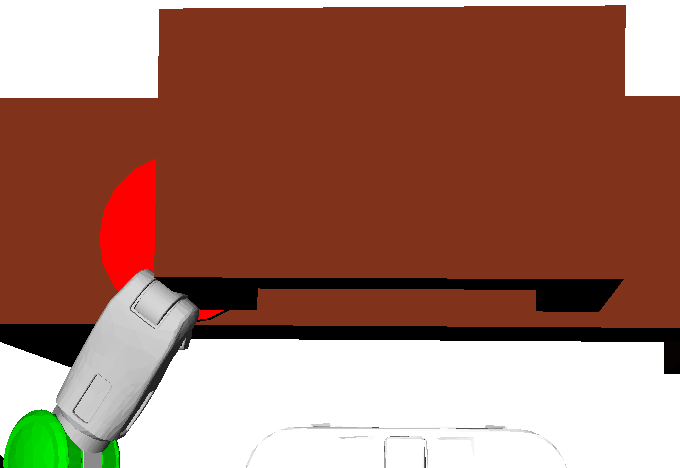
\includegraphics[scale=0.15]{images/fry_bad_grasp_pd1.png}\hspace{6mm}
%     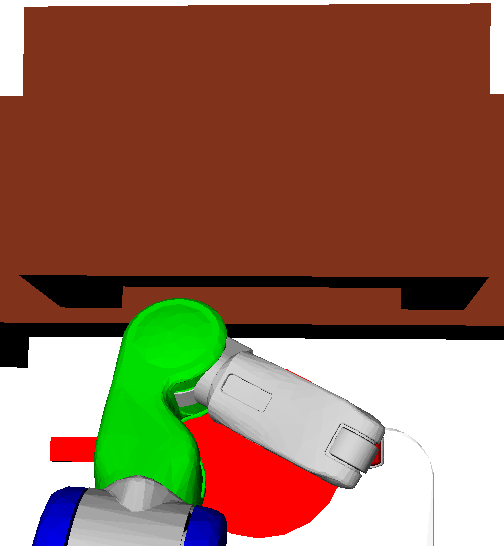
\includegraphics[scale=0.15]{images/fry_bad_grasp_pd2.png}
%     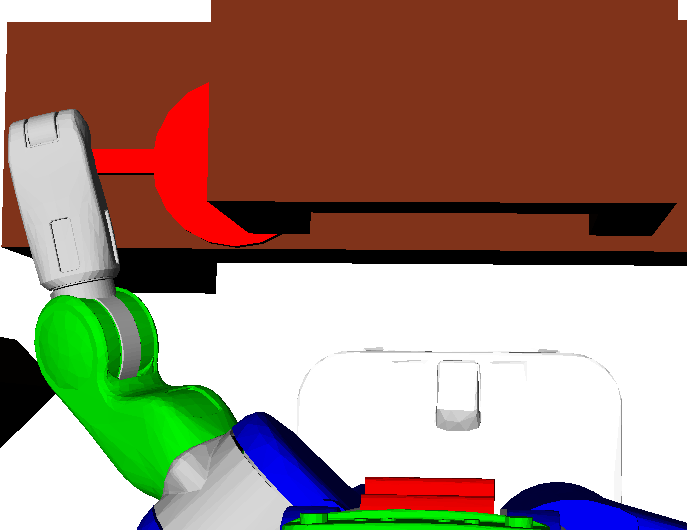
\includegraphics[scale=0.16]{images/fry_good_grasp_bad_pd.png}\hspace{6mm}
%     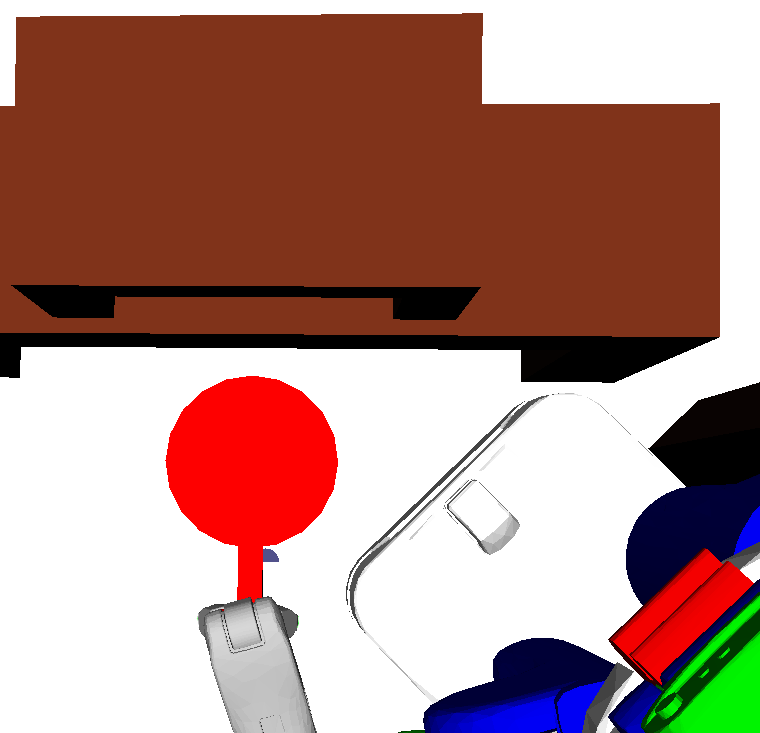
\includegraphics[scale=0.13]{images/fry_good_grasp_good_pd.png}
%   \caption{\small{\textbf{Top}: When the frying pan is not grasped by the handle, any attempted putdown pose for
% placing it into the narrow shelf fails. \textbf{Bottom}: When the frying pan is grasped by the handle, some putdown
% poses may succeed, as in the right, and some may fail, as in the left. In general, delayed rewards
% are important in the plan refinement {\sc mdp}; sometimes multiple symbolic references require resampling to
% change an infeasible refinement into a feasible one.}}
%   \label{fig:delayed}
% \end{figure}

\subsection{Training Process}
We learn a policy for this {\sc mdp} by adapting the method of Zucker et al.~\cite{workspacebias}, which
uses a linear combination of features to define a distribution over poses. In our setting, we learn a weight
vector $\theta_{p}$ for each reference \emph{type}, comprised of a pose type and possibly a gripper
(e.g., ``left gripper grasping pose,'' ``right gripper putdown pose,'' ``base pose'').
This decouples the learned distributions from any single high-level plan and allows generalization across problem instances.

We develop a feature function $f(s, a) = f(s, p, x)$ that maps the current
state $s \in \St$ and action $a \in \A$ to a
feature vector; $f$ defines a policy class for the {\sc mdp}. Additionally, we define
$N$ as the number of planning problems on which to train and
$\epsilon$ as the number of samples comprising a training episode, after which we update weights.

The training is a natural extension of randomized
refinement and progresses as follows. $N$ times, sample from $\Prob$ to obtain
a complete planning problem $\Pi$. For each $\Pi$, run the randomized refinement
algorithm to attempt to find a valid plan refinement, allowing the \textsc{Resample}
routine to be called $H$ times before termination. Select actions according to the $\theta_{p}$
and collect rewards according to $R$. After every $\epsilon$ calls to
\textsc{Resample}, perform a gradient update on the weights.

\subsection{Distribution and Gradient Updates}
We adopt the sampling distribution used in Zucker et al.~\cite{workspacebias}
for a symbolic reference $p$ with sample value $x$, in state $s \in \St$:
$$q(s, p, x) \propto \exp(\theta_{p}^{T} f(s, p, x)).$$
We define the expected reward of an episode $\xi$,
$$\eta(\theta_{p}) = \mathbb{E}_{q}[R(\xi)],$$ and approximate its gradient:
$$\nabla \eta(\theta_{p}) \approx \frac{R(\xi)}{\epsilon} \sum_{i=1}^{\epsilon}(f(s, p, x_{i}) - \mathbb{E}_{q,s}[f]).$$
$R(\xi)$ is the sum over all rewards obtained throughout $\xi$, and
$\mathbb{E}_{q,s}[f]$ is the expected feature vector under $q$ in state $s$. The weight vector update is then:
$$\theta_{p} \leftarrow \theta_{p} + \alpha \nabla \eta(\theta_{p})$$
for appropriate step size $\alpha$.

We sample $x$ from $q$ using the Metropolis algorithm~\cite{chib1995understanding}.
Since our distributions are continuous, calculating $\mathbb{E}_{q,s}[f]$ is hard,
so we approximate it with a Monte Carlo estimate.